\subsection{Gamma Spectroscopy}\label{gammaspectr}

The data from GALILEO rings were collected alongside the TRACE one during the
GALTRACE experiment. The spectrum of all the gamma rays that were observed,
can be visualized in Fig.~\ref{gamma}.
For a more precise analysis, it is possibile to consider the events for each
ring of the GALILEO detector sperately, even though, for an initial stage,
it is useful to look at the sum of gamma rays detected at each angle.
Moreover, gamma matrices were constructed through a C++ code,
implemented in ROOT environment, to search for the gamma coincidences.
This is necessary to observe different cascades of gamma emission for the
daughter nuclei produced in the experiment.
They can be seen in Fig.~\ref{matrix:F} and in Fig.~\ref{matrix:Li}.
The two plots differ in the Doppler correction: for the first it is supposed
that the mother nucleus is a \ce{^19 F}, for the second a \ce{^7 Li} one.

\begin{figure}[h]
  \centering
  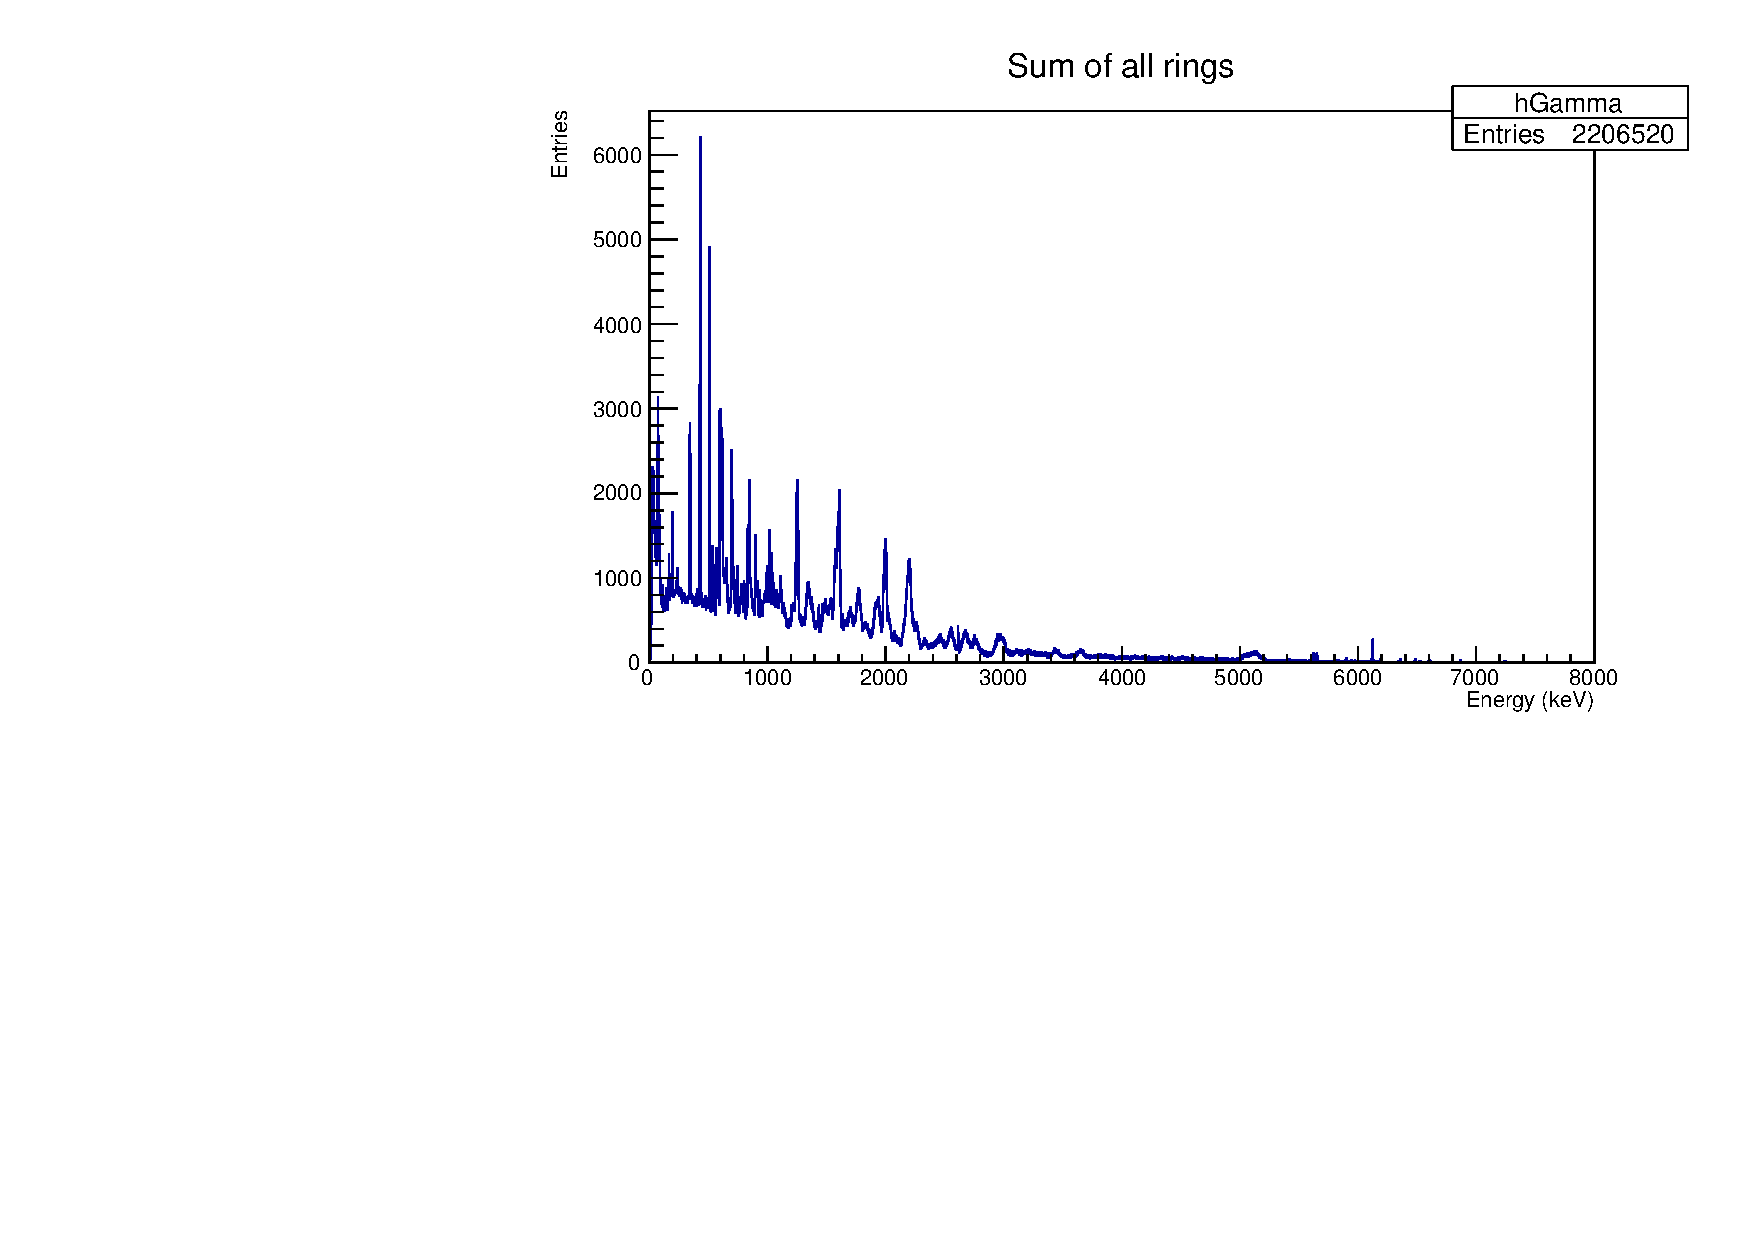
\includegraphics[scale=.6]{img/gamma.pdf}
  \caption{Gamma spectrum obtained from the sum of all GALILEO rings.}
  \label{gamma}
\end{figure}

\begin{figure}[h]
  \centering
  \begin{minipage}[b]{0.45\textwidth}
    \vspace{5mm}
    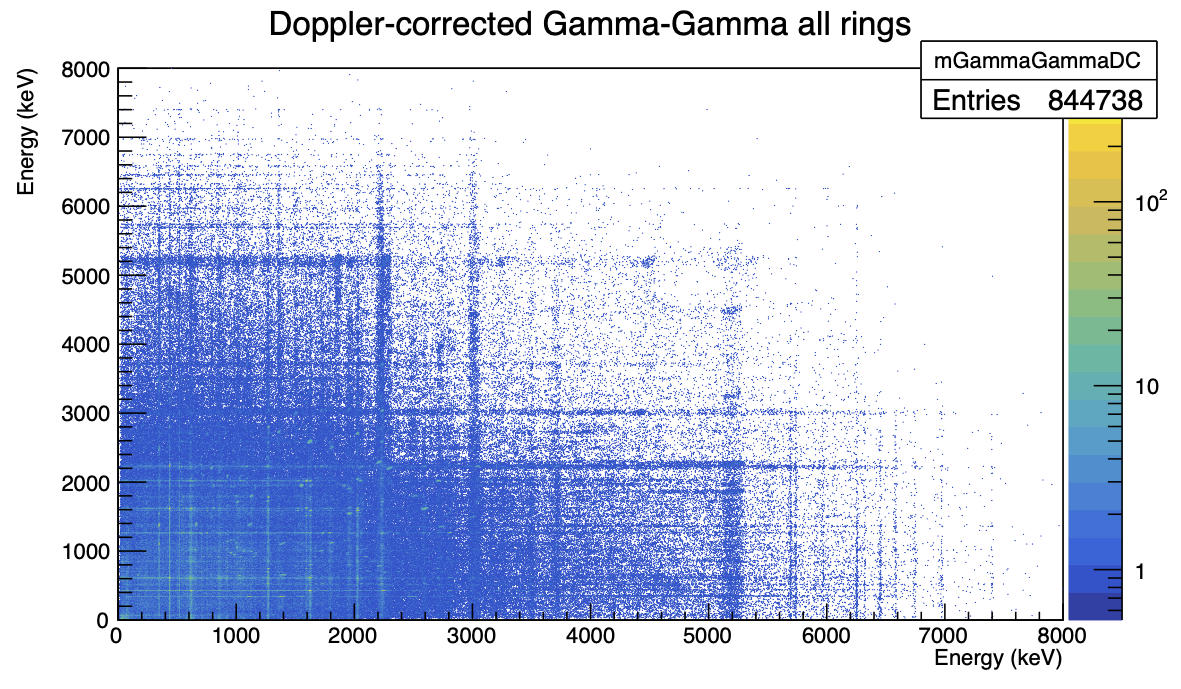
\includegraphics[width=\textwidth]{img/matrix_F.png}
    \caption{Gamma matrix for \ce{^19 F} Doppler correction.}
    \label{matrix:F}
  \end{minipage}
  \hfill
  \begin{minipage}[b]{0.45\textwidth}
    \vspace{5mm}
    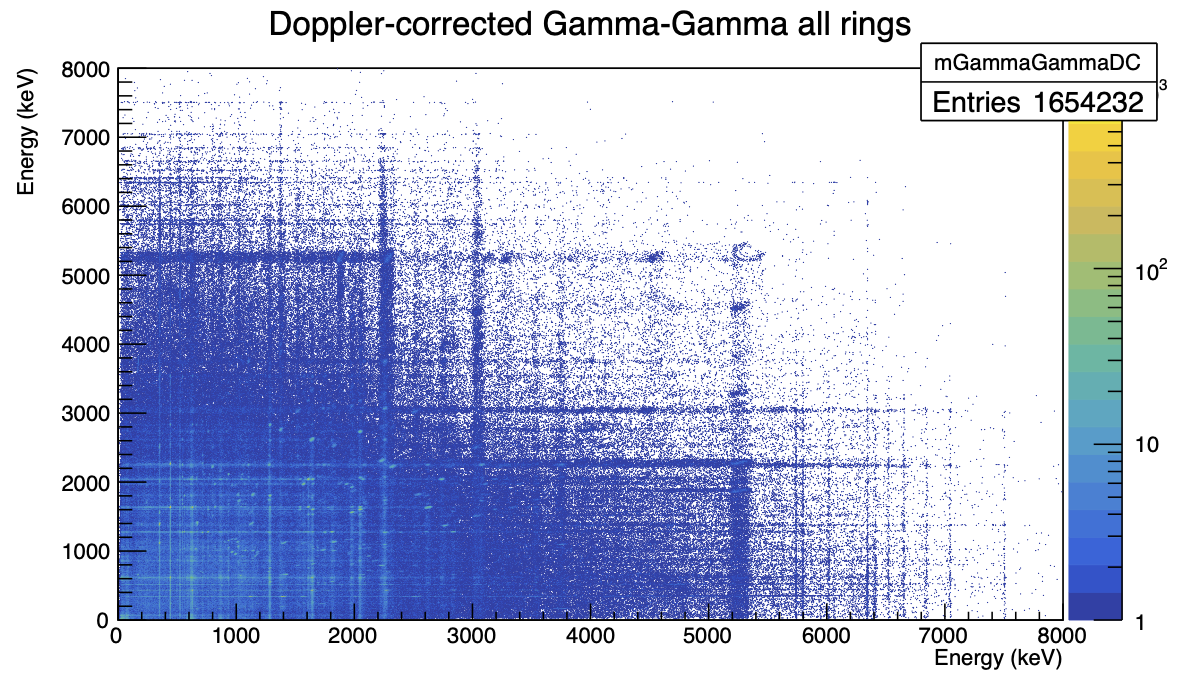
\includegraphics[width=\textwidth]{img/matrix_Li.png}
    \caption{Gamma matrix for \ce{^7 Li} Doppler correction.}
    \label{matrix:Li}
  \end{minipage}
\end{figure}

In order to look for a specific nuclei, simulations are made through PACE4 code
\cite{lise} implemented in LISE software. First one in case of a \ce{^7 Li}
and the second one in case of a \ce{^19 F} projectile.
In both cases the same Center of Mass energy was used (23 MeV) and
the same target (\ce{^12 C}). The expected abbundances of daughter nuclei
produced in the collissions are shown in Tab.~\ref{sim:F} and in
Tab.~\ref{sim:Li}.

\begin{figure}[h]
  \centering
  \begin{minipage}[b]{0.45\textwidth}
    \centering
  \begin{tabular}{ll}
    Daughter Nucleus & Percent \\
    \midrule
    \ce{^31 P} & \num{2.2}\% \\
    \ce{^31 Si} & \num{0.7}\% \\
    \ce{^30 P} & \num{22.6}\% \\
    \ce{^30 Si} & \num{14.3}\% \\
    \ce{^30 Al} & \num{0.7}\% \\
    \ce{^29 P} & \num{0.6}\% \\
    \ce{^29 Si} & \num{27.1}\% \\
    \ce{^29 Al} & \num{0.2}\% \\
    \ce{^28 Al} & \num{0.6}\% \\
    \ce{^27 Al} & \num{27.5}\% \\
    \ce{^27 Mg} & \num{2.4}\% \\
    \ce{^24 Na} & \num{1}\% \\
    \ce{^23 Na} & \num{0.1}\% \\
    \bottomrule
  \end{tabular}
  \caption{Yields of daughter nuclei for \ce{^19 F}.}
  \label{sim:F}
  \end{minipage}
  \hfill
  \begin{minipage}[b]{0.45\textwidth}
    \centering
  \begin{tabular}{ll}
    Daughter Nucleus & Percent \\
    \midrule
    \ce{^19 F} & \num{7.3}\% \\
    \ce{^19 O} & \num{3.2}\% \\
    \ce{^18 F} & \num{0.2}\% \\
    \ce{^18 O} & \num{8.3}\% \\
    \ce{^16 N} & \num{0.1}\% \\
    \ce{^15 N} & \num{80.7}\% \\
    \ce{^15 C} & \num{0.2}\% \\
    \bottomrule
  \end{tabular}
  \caption{Yields of daughter nuclei for \ce{^7 Li}.}
  \label{sim:Li}
  \end{minipage}
\end{figure}

\bigbreak

Matrices present a high number of background events, thus the next step should
consists in taking advantage of the NN output variables. As some of the
reactions (i.e.\ \ce{^18 O} production) involves emission of a proton or an
$\alpha$, it is possibile to clean the GALILEO gamma matrices taking into
account only the events in which a particle is detected by the TRACE detector.
Such a step is still in the making by the GALTRACE collaboration, and is not
in the interest of this report.
